La phase de conception du sprint 1.2 débute par l’élaboration du diagramme de classes, suivi de diagrammes de séquence représentant divers cas d'utilisation. 

\subsubsection{Diagramme de classe du sprint 1.2}
Ce diagramme vise à modéliser les principales entités métier du système, leurs attributs, leurs méthodes ainsi que les relations existantes entre elles.

La figure \ref{fig:classsp1} présente le diagramme de classes correspondant à ce sprint.
\begin{figure}[H]
    \centering
    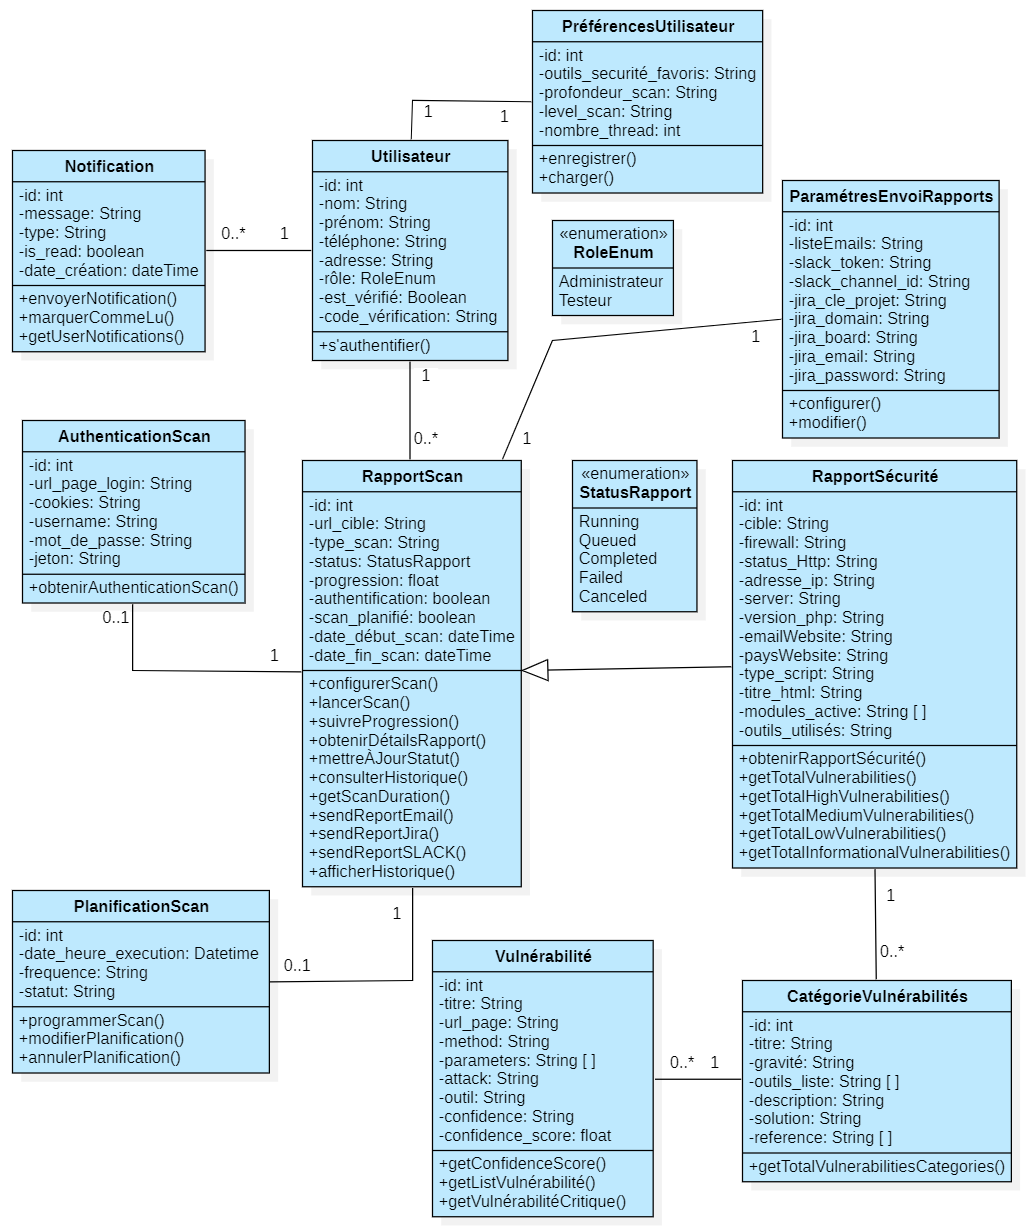
\includegraphics[width=0.9\linewidth]{chapitres/ch3Sp1/section/sprint2/img/classeL1-SP1.2.png}
    \caption{Diagramme de classe du sprint 1.2}
    \label{fig:classsp1}
\end{figure}
\vspace{-0.6cm}
Les principales classes modélisées sont les suivantes :
\begin{itemize}[label=$*$]
    \item \textbf{Utilisateur} : Représente un utilisateur de l’application.
    \item \textbf{PréférencesUtilisateur} : Contient les préférences techniques d’un utilisateur pour les scans (profondeur, niveau, nombre de threads, outils favoris), associée de manière 1-à-1 avec la classe \texttt{Utilisateur}.
    
    \item \textbf{Notification} : Gère les notifications envoyées aux utilisateurs, avec des attributs comme le message, le type et la date de création. Un utilisateur peut recevoir plusieurs notifications.
    
    \item \textbf{ParametresEnvoiRapports} : Stocke les paramètres nécessaires pour l’envoi des rapports (emails, Slack, Jira), incluant les jetons, identifiants et adresses associées à chaque canal de communication.
    
    \item \textbf{RapportScan} : Regroupe les données liées à un scan de sécurité, comme le type de scan, son état (via \texttt{StatusRapport}), la cible, les dates de début/fin, les outils utilisés... Cette classe contient également des méthodes pour configurer, lancer et suivre un scan.
    
    \item \textbf{AuthenticationScan} : Contient les informations nécessaires pour effectuer un scan authentifié (page de login, identifiants, cookies, jetons). Un rapport de scan peut avoir 0 ou 1 configuration d’authentification.
    \item \textbf{RapportSecurite} : Fournit des détails techniques sur l’environnement cible d’un scan : en-têtes HTTP, serveur, version PHP, adresse IP, pays d’hébergement, titre HTML, etc.
    \item \textbf{PlanificationScan} : Permet de planifier l’exécution automatique d’un scan à une date donnée avec une fréquence spécifique. Elle offre des méthodes de gestion comme la mise à jour ou l’annulation d’un scan planifié. Un scan peut être associé à une planification. 
    \item \textbf{Vulnérabilité} : Décrit une vulnérabilité détectée, avec ses détails techniques (type d’attaque, méthode HTTP, paramètres concernés, gravité, score de confiance...) avec des méthodes pour calculer le nombre de vulnérabilités par criticité..
    \item \textbf{CatégorieVulnérabilités} : Catégorise les vulnérabilités détectées selon leur nature, leur niveau de risque, les outils les ayant détectées, la description,  la solution recommandée... Une catégorie peut regrouper plusieurs vulnérabilités.
    \item \textbf{StatusRapport (Énumération)} : Représente l’état d’avancement d’un rapport de scan. Les valeurs possibles sont : \texttt{Running}, \texttt{Queued}, \texttt{Completed}, \texttt{Failed}, et \texttt{Canceled}.
\end{itemize}
Les associations entre classes sont également représentées dans le diagramme, notamment:
\begin{itemize}[label=$-$]
    \item Un \texttt{utilisateur} peut recevoir plusieurs \texttt{notifications}.
    \item Un \texttt{rapport de scan} peut être lié à une ou plusieurs \texttt{vulnérabilités} et appartenir à une \texttt{catégorie} donnée.
    \item Un \texttt{scan} peut être planifié via la classe \texttt{"PlanificationScan"}.
    \item Un \texttt{rapport de sécurité} est généralement associé à un scan donné.
\end{itemize}
Ce diagramme constitue une base essentielle pour la suite du développement, en assurant une structure cohérente et maintenable du code tout au long des itérations agiles.

\subsubsection{Diagramme de séquence de conception}
Les diagrammes de séquence visant à décrire dynamiquement l’enchaînement des interactions entre objets pour différents cas d'utilisation.

\textbf{Diagramme de séquence de conception de cas «Lancer un scan de test sécurité»}:\\
Le diagramme présenté illustre le processus de lancement d’un scan de test de sécurité à travers l'interaction des différents composants du système.
\begin{itemize}[label=$-$]
    \item \textbf{Lancement du scan:} L’utilisateur initie un scan via l’interface. Le backend (FastAPI) reçoit la requête, crée une nouvelle entrée dans la base de données avec le statut \textit{"pending"}, et publie la tâche de scan dans la file RabbitMQ en incluant l'identifiant du scan.
    \item \textbf{Mise en file d’attente:} Si un worker (processus de traitement) est disponible, il récupère la tâche. Si aucun worker n’est libre (file pleine), la tâche est mise en attente. Le statut du scan est alors mis à jour à \textit{"queued"}, une notification d’attente est envoyée via WebSocket, et un message d’attente est affiché à l’utilisateur.
    \item \textbf{Exécution du scan:} Dès qu’un worker devient disponible, le scan passe au statut \textit{"running"}. L’exécution des outils de pentest démarre (en mode multithread via la classe \texttt{GestionnairePentestClass}). Le backend met à jour le pourcentage de progression dans la base de données, et ces informations sont transmises en temps réel à l’interface utilisateur via WebSocket.
    \item \textbf{Détection de vulnérabilités critiques:} Si des vulnérabilités critiques sont identifiées, elles sont envoyées via WebSocket à l’utilisateur en temps réel et affichées immédiatement.
    \item \textbf{Finalisation du scan:} Une fois l’analyse terminée, les résultats et le rapport sont enregistrés dans la base de données. Le statut du scan est mis à jour à \textit{"completed"}, et le rapport final est envoyé à l’utilisateur pour affichage.
\end{itemize}

Ce mécanisme asynchrone, reposant sur RabbitMQ et une architecture multithreadée, permet de gérer plusieurs scans simultanément tout en assurant une communication en temps réel avec l’utilisateur.
\begin{figure}[H]
    \centering
    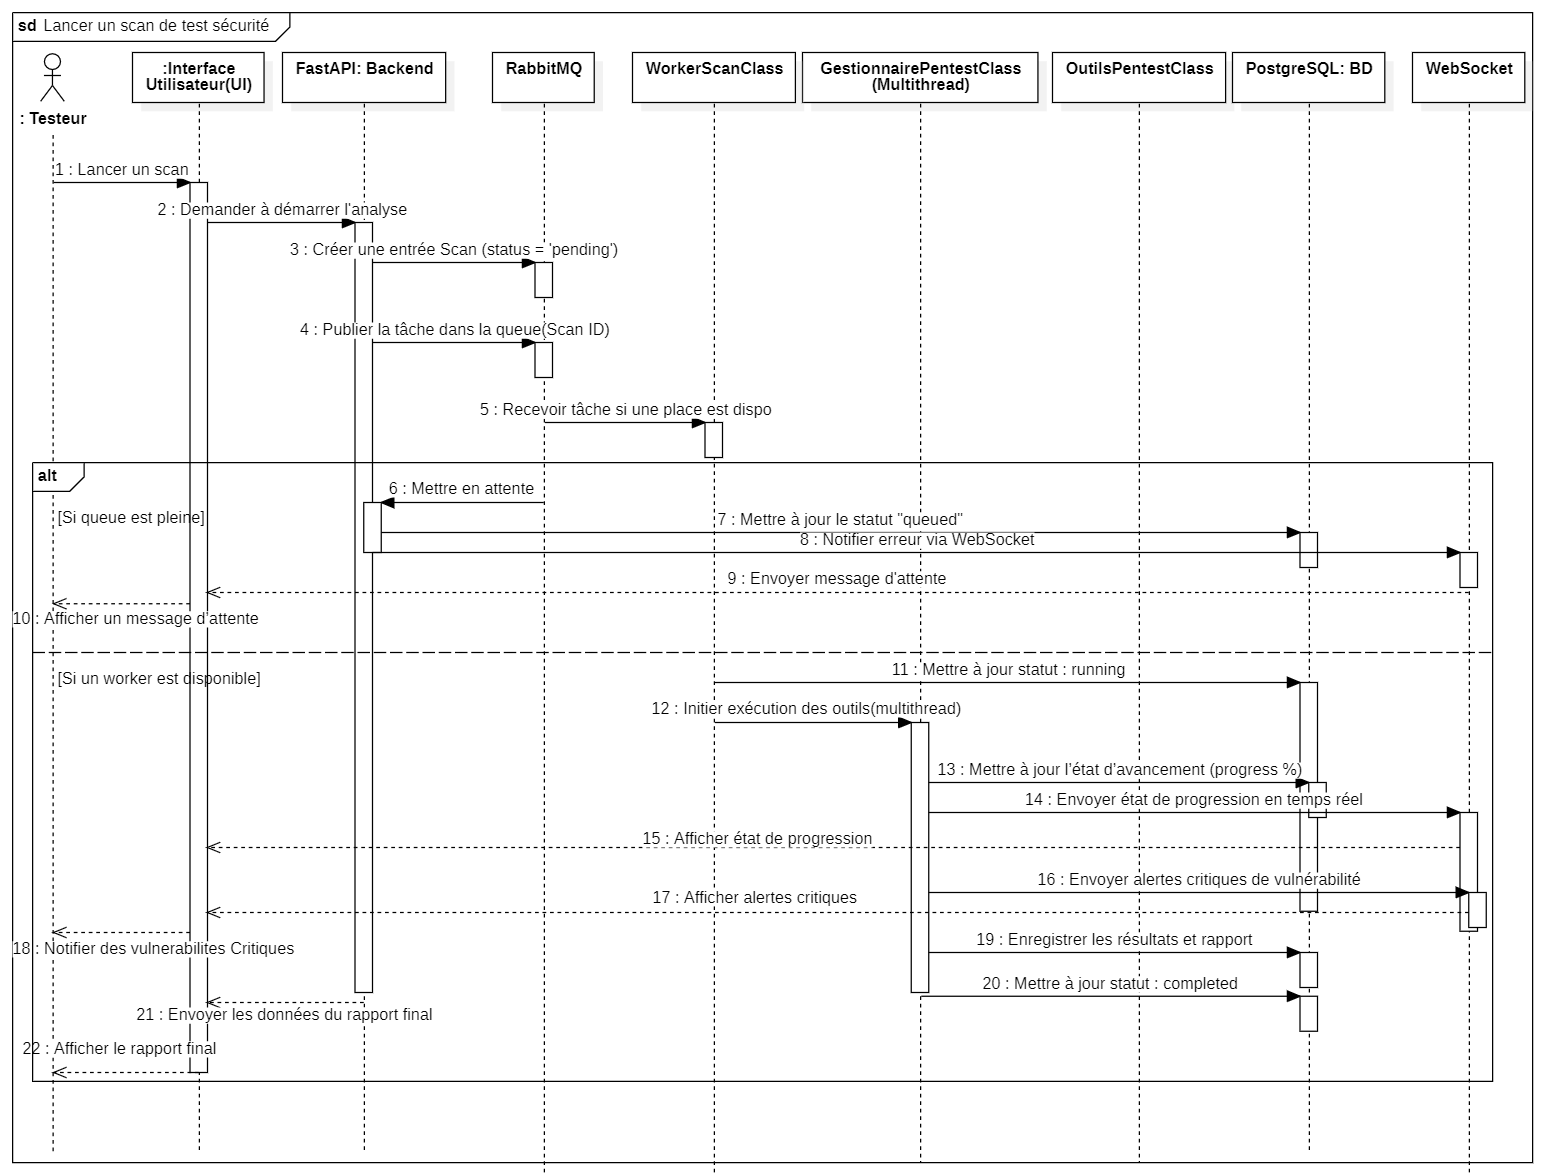
\includegraphics[width=\linewidth]{chapitres/ch3Sp1/section/sprint2/img/seq-lancerSp1.2.png}
    \caption{\centering Diagramme de séquence de conception de cas «Lancer un scan de test sécurité»}
    \label{fig:seq1ScanAnalyse}
\end{figure}
\vspace{-0.6cm}
